% govsmart_fig2.tex — Standalone two-panel figure for GovSmart paper
% Panel (a): Stacked horizontal bar chart — task completion breakdown
% Panel (b): Vertical bar chart — execution duration (median + range)
\documentclass[border=6pt]{standalone}
\usepackage[T1]{fontenc}
\usepackage{pgfplots}
\pgfplotsset{compat=1.18}
\usepackage{xcolor}

% --- colour palette (forest / amber / brick) ---
\definecolor{cS}{HTML}{2E7D32}   % Success (S) — green
\definecolor{cSH}{HTML}{F9A825}  % Success with help (SH) — amber
\definecolor{cF}{HTML}{C62828}   % Failure (F) — red
\definecolor{cBar}{HTML}{1565C0} % Duration bars — blue
\definecolor{cTimeout}{HTML}{C62828} % Timeout line

\begin{document}
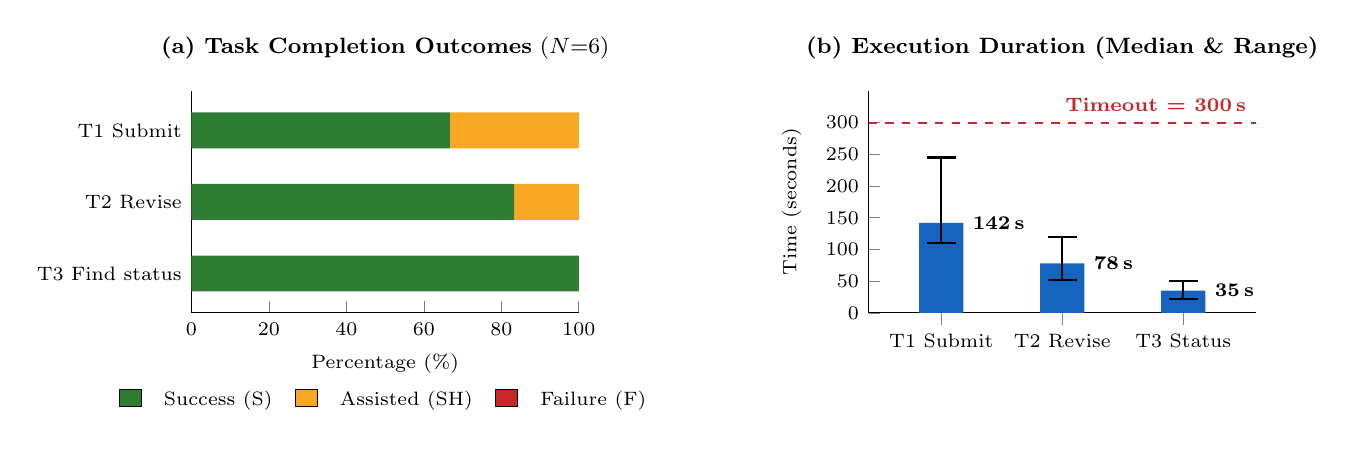
\begin{tikzpicture}
% =========================================================================
% === PANEL (A): Task Completion Outcomes ===
% =========================================================================
\begin{axis}[
    name=axA,
    at={(0cm, 0cm)},
    title={\textbf{(a) Task Completion Outcomes} ($N{=}6$)},
    title style={font=\footnotesize, yshift=2pt},
    xbar stacked,
    width=6.5cm, height=4.4cm,
    bar width=13pt,
    xmin=0, xmax=100,
    xlabel={Percentage (\%)},
    xlabel style={font=\scriptsize},
    ytick={1,2,3},
    yticklabels={T3 Find status, T2 Revise, T1 Submit},
    yticklabel style={font=\scriptsize, anchor=east},
    xticklabel style={font=\scriptsize},
    legend style={
        at={(0.5,-0.30)},
        anchor=north,
        legend columns=3,
        font=\scriptsize,
        draw=none,
        column sep=6pt,
    },
    enlarge y limits={abs=0.55},
    axis lines*=left,
    clip=false,
    set layers,
]
% S segments
\addplot[fill=cS, draw=none] coordinates {(100,1) (83.3,2) (66.7,3)};
% SH segments
\addplot[fill=cSH, draw=none] coordinates {(0,1) (16.7,2) (33.3,3)};
% F segments (all zero)
\addplot[fill=cF, draw=none] coordinates {(0,1) (0,2) (0,3)};

% percentage labels inside bars
\node[font=\scriptsize\bfseries, white] at (axis cs:33.3,3) {66.7\%};
\node[font=\scriptsize\bfseries] at (axis cs:83.3,3) {33.3\%};
\node[font=\scriptsize\bfseries, white] at (axis cs:41.7,2) {83.3\%};
\node[font=\scriptsize\bfseries] at (axis cs:91.7,2) {16.7\%};
\node[font=\scriptsize\bfseries, white] at (axis cs:50,1) {100\%};

\legend{Success (S), Assisted (SH), Failure (F)}
\end{axis}

% =========================================================================
% === PANEL (B): Execution Duration (Median & Range) ===
% =========================================================================
\begin{axis}[
    name=axB,
    at={(8.6cm, 0cm)},
    title={\textbf{(b) Execution Duration (Median \& Range)}},
    title style={font=\footnotesize, yshift=2pt},
    ybar,
    width=6.5cm, height=4.4cm,
    bar width=16pt,
    ymin=0, ymax=350,
    ylabel={Time (seconds)},
    ylabel style={font=\scriptsize, yshift=2pt},
    xtick={1,2,3},
    xticklabels={T1 Submit, T2 Revise, T3 Status},
    xticklabel style={font=\scriptsize},
    yticklabel style={font=\scriptsize},
    enlarge x limits={abs=0.6},
    axis lines*=left,
    clip=false,
    ytick={0,50,100,150,200,250,300},
]
% Median bars
\addplot[fill=cBar, draw=none] coordinates {(1,142) (2,78) (3,35)};

% Error bars (range: min to max)
% T1: 110–245, median 142
\draw[thick, black] (axis cs:1,110) -- (axis cs:1,245);
\draw[thick, black] (axis cs:0.88,110) -- (axis cs:1.12,110);
\draw[thick, black] (axis cs:0.88,245) -- (axis cs:1.12,245);

% T2: 52–120, median 78
\draw[thick, black] (axis cs:2,52) -- (axis cs:2,120);
\draw[thick, black] (axis cs:1.88,52) -- (axis cs:2.12,52);
\draw[thick, black] (axis cs:1.88,120) -- (axis cs:2.12,120);

% T3: 22–50, median 35
\draw[thick, black] (axis cs:3,22) -- (axis cs:3,50);
\draw[thick, black] (axis cs:2.88,22) -- (axis cs:3.12,22);
\draw[thick, black] (axis cs:2.88,50) -- (axis cs:3.12,50);

% Median labels — placed cleanly to the right of error bars
\node[font=\scriptsize\bfseries, anchor=west] at (axis cs:1.18,142) {142\,s};
\node[font=\scriptsize\bfseries, anchor=west] at (axis cs:2.18,78) {78\,s};
\node[font=\scriptsize\bfseries, anchor=west] at (axis cs:3.18,35) {35\,s};

% Timeout dashed line at y=300 with label
\draw[cTimeout, dashed, thick] (axis cs:0.4,300) -- (axis cs:3.6,300);
\node[font=\scriptsize\bfseries, cTimeout, anchor=south east] at (axis cs:3.6,302) {Timeout = 300\,s};

\end{axis}
\end{tikzpicture}
\end{document}
